\chapter{Статические магнитоэлектрические эффекты}\label{ch:ch2}

В данной главе анализируются экспериментальные данные по магнитоэлектрической связи ионов меди и никеля в \ncbo, полученные в работах \cite{Nenert2007, Khan2013} (см. \cref{sec:ch1/sec2}). Объясняется, почему авторы \cite{Nenert2007} не смогли обнаружить индукции электрической поляризации при переходе чистого \cbo\ в антиферромагнитную фазу и почему это удалось сделать в соединении, допированном ионами \niIon.

\section{Расчет расщепления состояний \cud\ и \nif\ кристаллическим полем}\label{sec:ch2/sec1}

\begin{figure}[ht]
    \centerfloat{
        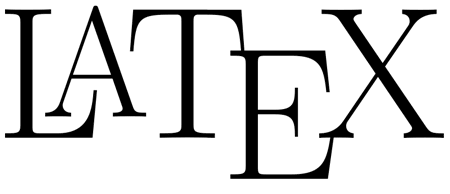
\includegraphics[scale=0.27]{latex}
    }
    \caption{TeX.}\label{fig:latex}
\end{figure}



\FloatBarrier
